%%%%%%%%%%%%%%%%%%%%%%%%%%%%%%%%%%%%%%%%%
% Beamer Presentation
% LaTeX Template
% Version 1.0 (10/11/12)
%
% This template has been downloaded from:
% http://www.LaTeXTemplates.com
%
% License:
% CC BY-NC-SA 3.0 (http://creativecommons.org/licenses/by-nc-sa/3.0/)
%
%%%%%%%%%%%%%%%%%%%%%%%%%%%%%%%%%%%%%%%%%

%----------------------------------------------------------------------------------------
% PACKAGES AND THEMES
%----------------------------------------------------------------------------------------

\documentclass[10pt,xcolor={dvipsnames}]{beamer}
%\setbeamersize{text margin left=1em,text margin right=1em}
\usepackage{mathtools}
\usepackage{amsmath}
\usepackage{bm}
\usepackage{hyperref}

\usepackage{graphicx} % Allows including images
\graphicspath{{/Users/rebecca/Documents/Rivet_Analyses/MC_VBFDM/PlotCombinationTool/Figures/}{/Users/rebecca/Documents/Presentations/Talks/}{/Users/rebecca/Documents/Rivet_Analyses/MC_VBFDM/PlotCombinationTool/Figures/StatPlots/}{/Users/rebecca/Documents/Rivet_Analyses/MC_VBFDM/PlotCombinationTool/Figures/2DHists/}}
\usepackage{booktabs} % Allows the use of \toprule, \midrule and \bottomrule in tables

\usepackage{etoolbox}

\usepackage{subcaption}
\captionsetup{compatibility=false}

\usepackage{multirow}

\usepackage{appendixnumberbeamer}

%\newlength\origleftmargini
%\setlength\origleftmargini\leftmargini
%\setbeamertemplate{itemize/enumerate body begin}{\setlength{\leftmargini}{2pt}}%

%\let\oldexampleblock\exampleblock
%\let\oldendexampleblock\endexampleblock
%\def\exampleblock{\begingroup \setbeamertemplate{itemize/enumerate body begin}{\setlength{\leftmargini}{\origleftmargini}} \oldexampleblock}
%\def\endexampleblock{\oldendexampleblock \endgroup}%

%\let\oldalertblock\alertblock
%\let\oldendalertblock\endalertblock
%\def\alertblock{\begingroup \setbeamertemplate{itemize/enumerate body begin}{\setlength{\leftmargini}{\origleftmargini}} \oldalertblock}
%\def\endalertblock{\oldendalertblock \endgroup}

\mode<presentation> {

% The Beamer class comes with a number of default slide themes
% which change the colors and layouts of slides. Below this is a list
% of all the themes, uncomment each in turn to see what they look like.

%\usetheme{default}
%\usetheme{AnnArbor}
%\usetheme{Antibes}
%\usetheme{Bergen}
%\usetheme{Berkeley}
%\usetheme{Berlin}
\usetheme{Boadilla}
%\usetheme{CambridgeUS}
%\usetheme{Copenhagen}
%\usetheme{Darmstadt}
%\usetheme{Dresden}
%\usetheme{Frankfurt}
%\usetheme{Goettingen}
%\usetheme{Hannover}
%\usetheme{Ilmenau}
%\usetheme{JuanLesPins}
%\usetheme{Luebeck}
%\usetheme{Madrid}
%\usetheme{Malmoe}
%\usetheme{Marburg}
%\usetheme{Montpellier}
%\usetheme{PaloAlto}
%\usetheme{Pittsburgh}
%\usetheme{Rochester}
%\usetheme{Seahorse}
%\usetheme{Singapore}
%\usetheme{Szeged}
%\usetheme{Warsaw}

% As well as themes, the Beamer class has a number of color themes
% for any slide theme. Uncomment each of these in turn to see how it
% changes the colors of your current slide theme.

%\usecolortheme{albatross}
%\usecolortheme{beaver}
%\usecolortheme{beetle}
%\usecolortheme{crane}
%\usecolortheme{dolphin}
%\usecolortheme{dove}
%\usecolortheme{fly}
%\usecolortheme{lily}
%\usecolortheme{RoyalBlue}
%\usecolortheme{rose}
%\usecolortheme{seagull}
%\usecolortheme{seahorse}
%\usecolortheme{whale}
%\usecolortheme{wolverine}

%%Changing the theme colours
%\setbeamercolor*{structure}{bg=Plum!20,fg=Plum}
%\setbeamercolor*{palette primary}{use=structure,fg=white,bg=structure.fg}
%\setbeamercolor*{palette secondary}{use=structure,fg=white,bg=structure.fg!75}
%\setbeamercolor*{palette tertiary}{use=structure,fg=white,bg=structure.fg!50!black}
%\setbeamercolor*{palette quaternary}{fg=white,bg=black}
%\setbeamercolor{section in toc}{fg=black,bg=white}
%%\setbeamercolor{alerted text}{use=structure,fg=structure.fg!50!black!80!black}
%\setbeamercolor{titlelike}{parent=palette primary,fg=structure.fg!50!black}
%\setbeamercolor{frametitle}{bg=gray!30!white,fg=Plum}
%\setbeamercolor*{titlelike}{parent=palette primary}

%Changing the theme colours
\setbeamercolor*{structure}{bg=RoyalPurple,fg=RoyalPurple}
\setbeamercolor*{palette primary}{use=structure,fg=white,bg=structure.fg}
\setbeamercolor*{palette secondary}{use=structure,fg=white,bg=structure.fg}
\setbeamercolor*{palette tertiary}{use=structure,fg=white,bg=structure.fg}
\setbeamercolor*{palette quaternary}{fg=white,bg=black}
\setbeamercolor{section in toc}{fg=black,bg=white}
%\setbeamercolor{alerted text}{use=structure,fg=structure.fg!50!black!80!black}
\setbeamercolor{titlelike}{parent=palette primary,fg=structure.fg!50!black}
%\setbeamercolor{frametitle}{use=structure,fg=white,bg=structure.fg}
\setbeamercolor*{titlelike}{parent=palette primary}

%\setbeamercolor{block}{bg=yellow!10,fg=black}
%\setbeamercolor{block title}{bg=yellow!50,fg=black}
%\AtBeginEnvironment{block}{\setbeamercolor{itemize item}{fg=yellow}}

\newenvironment<>{examplefirst}[1]{%
  \setbeamercolor{block title}{bg=yellow!50,fg=black}%
  \begin{block}#2{#1}}{\end{block}}
\AtBeginEnvironment{examplefirst}{\setbeamercolor{itemize item}{fg=yellow}}

%\setbeamertemplate{footline} % To remove the footer line in all slides uncomment this line
%\setbeamertemplate{footline}[page number] % To replace the footer line in all slides with a simple slide count uncomment this line

%\setbeamertemplate{navigation symbols}{} % To remove the navigation symbols from the bottom of all slides uncomment this line


\setbeamertemplate{blocks}[rounded][shadow=false]
\setbeamertemplate{itemize items}[circle]
\setbeamertemplate{itemize subitems}[circle]

\renewcommand{\thefootnote}{\alph{footnote}}

}

%----------------------------------------------------------------------------------------
% TITLE PAGE
%----------------------------------------------------------------------------------------



\title[VBFDM Statistical Test]{Statistical test for VBF DM observables} % The short title appears at the bottom of every slide, the full title is only on the title page

\author{\underline{Rebecca Pickles}, Darren Price} % Your name
%\institute[UoM] % Your institution as it will appear on the bottom of every slide, may be shorthand to save space
%{
%University of Manchester\\ % Your institution for the title page
%\medskip
%\textit{julia.iturbe@cern.ch} % Your email address
%}
% logo of my university
\titlegraphic{
\includegraphics[width=3cm]{UniOfManchesterLogo}}
\date{\today} % Date, can be changed to a custom date

\begin{document}

\begin{frame}
\titlepage % Print the title page as the first slide
\end{frame}

\iffalse
\begin{frame}
\frametitle{Overview} % Table of contents slide, comment this block out to remove it
\tableofcontents % Throughout your presentation, if you choose to use \section{} and \subsection{} commands, these will automatically be printed on this slide as an overview of your presentation
\end{frame}
\fi
%----------------------------------------------------------------------------------------
% PRESENTATION SLIDES
%----------------------------------------------------------------------------------------

%------------------------------------------------
\section{Introduction} % Sections can be created in order to organize your presentation into discrete blocks, all sections and subsections are automatically printed in the table of contents as an overview of the talk

%------------------------------------------------
\iffalse
\fi

\begin{frame}
\frametitle{Status}
\begin{itemize}
\item Constructed code to compare the DM VBF models (with the corrected data ratio from Emily and Zara):
\begin{itemize}
\item Ratio plots
\item $\chi^{2}$ statistical test (With room to adapt for different - more robust - test)
\end{itemize}
\item Compared DM models with the corrected ratios for Mjj
\item Produced 2D plots of Mjj vs $\delta\eta$
\end{itemize}
\end{frame}

\begin{frame}
\frametitle{Reminder of DM models}
\begin{columns}
\begin{column}{.3\textwidth} 
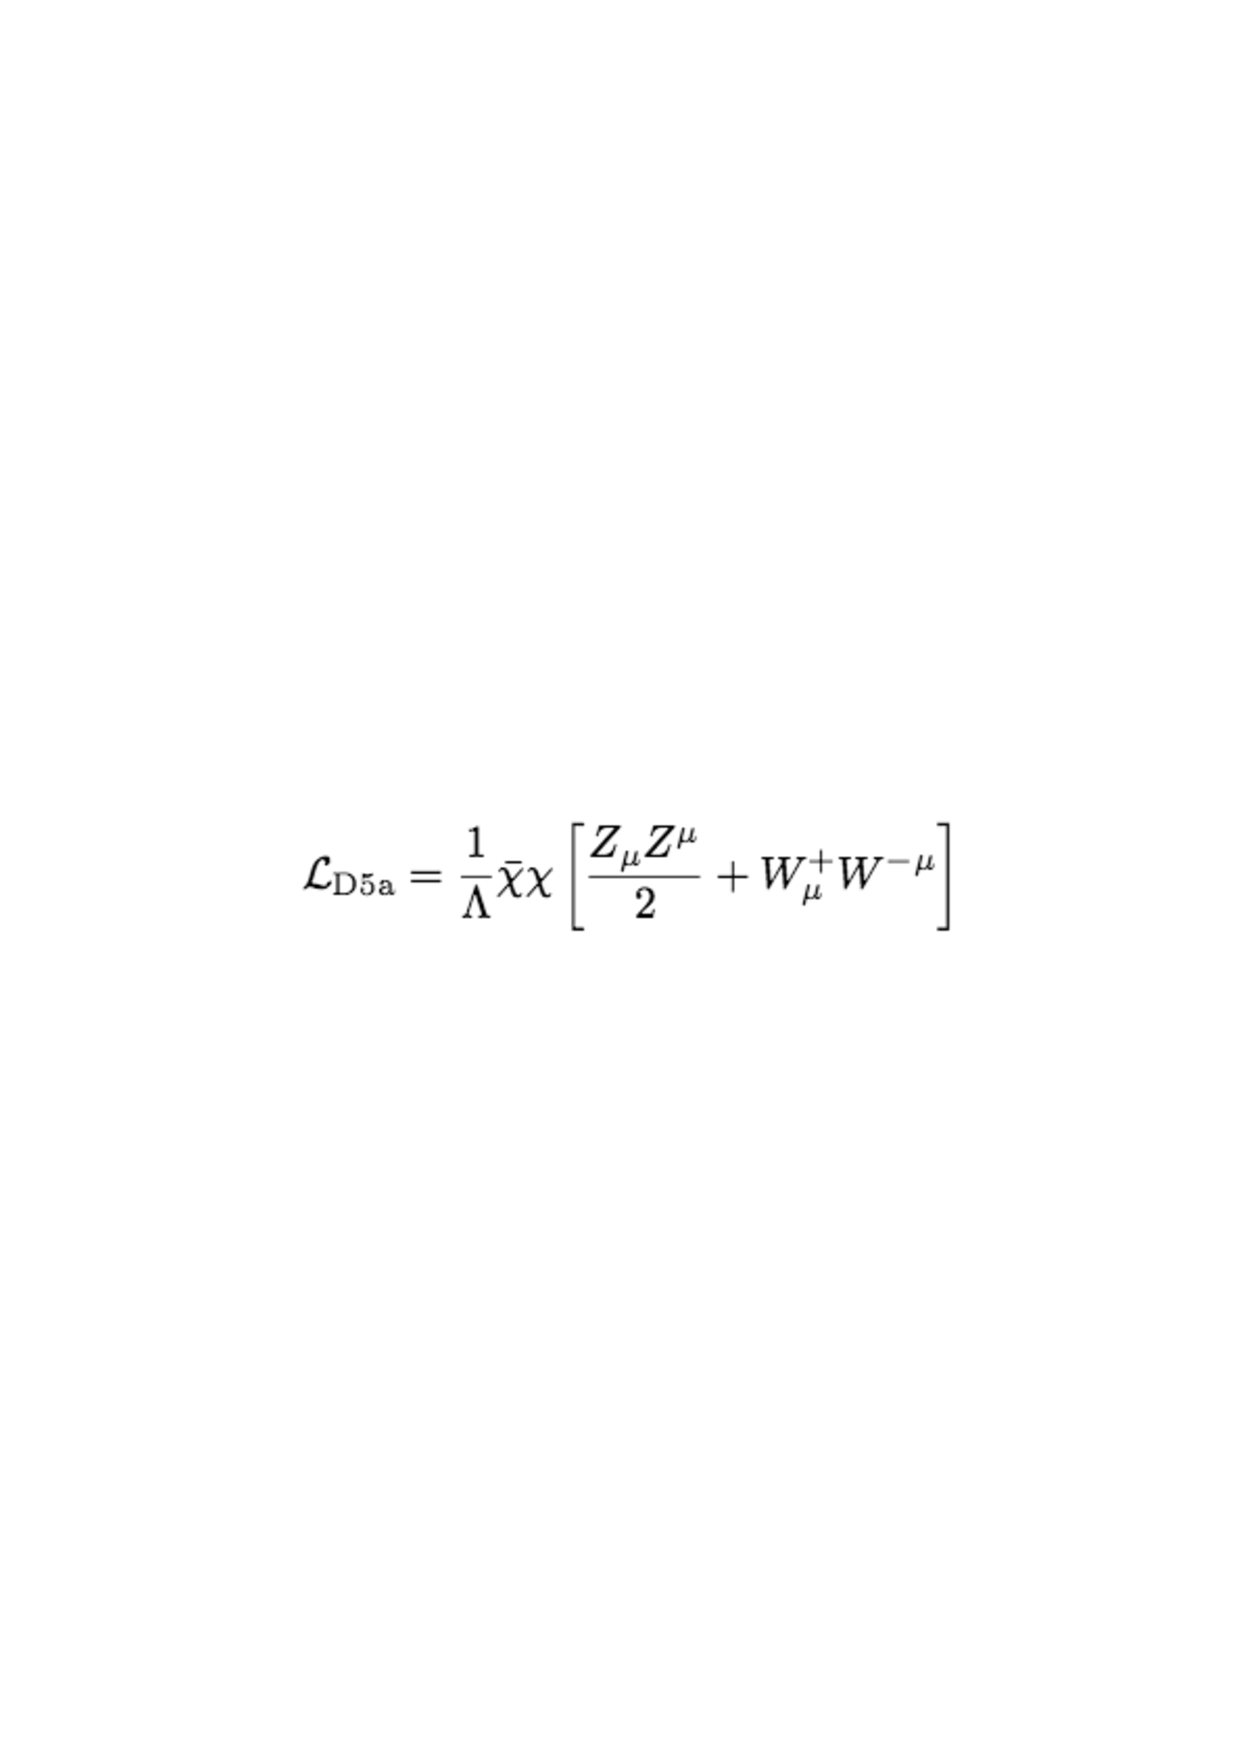
\includegraphics[width=4cm]{D5a_Lagrangian}
\newline \newline
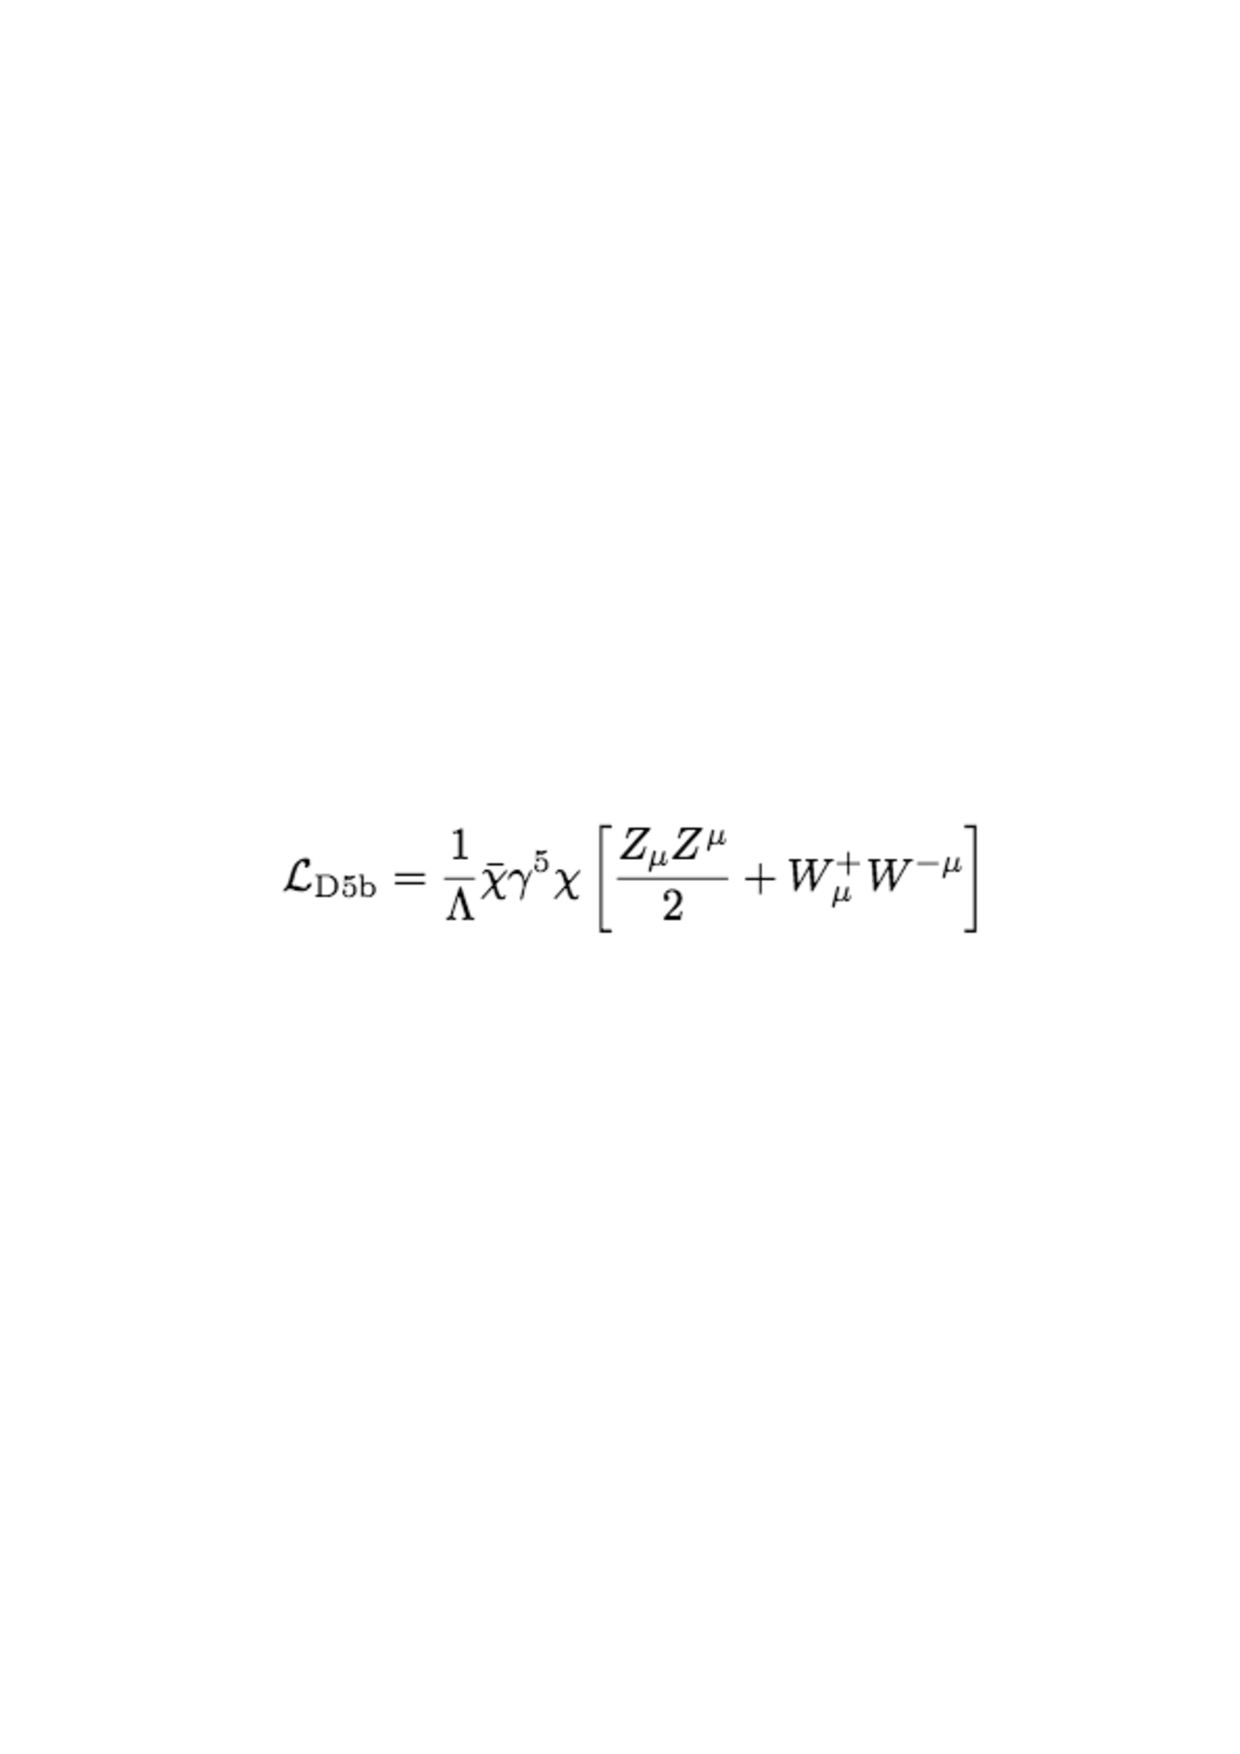
\includegraphics[width=4cm]{D5b_Lagrangian}
\newline \newline
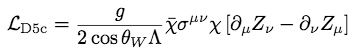
\includegraphics[width=4cm]{D5c_Lagrangian}
\end{column}
\begin{column}{.3\textwidth}
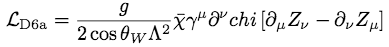
\includegraphics[width=4cm]{D6a_Lagrangian}
\newline \newline
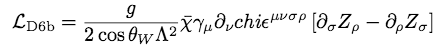
\includegraphics[width=4cm]{D6b_Lagrangian}
\newline \newline
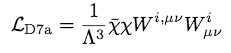
\includegraphics[width=4cm]{D7a_Lagrangian}
\end{column}
\begin{column}{.3\textwidth}
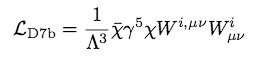
\includegraphics[width=4cm]{D7b_Lagrangian}
\newline \newline
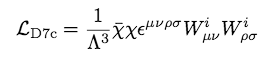
\includegraphics[width=4cm]{D7c_Lagrangian}
\newline \newline
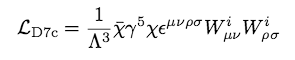
\includegraphics[width=4cm]{D7d_Lagrangian}
\end{column}
\end{columns}
\begin{itemize}
\item DM Mass and Lagrangian term influences the rates and kinematics.
\item Can study Higgs 'dark portal' where the interactions are the same as the BSM EFT
\item The different dimensions have the EFT constraints:
\begin{itemize}
\item D5c : $\Lambda$ = 3.3 TeV
\item D5d : $\Lambda$ = 6.6 TeV
\item D6a : $\Lambda$ = 230 GeV
\item D6b : $\Lambda$ = 330 GeV
\item This has meant that some dimensions would not be seen by any parameters
\end{itemize}
\end{itemize}
\end{frame}


\begin{frame}
\frametitle{(Z$\rightarrow\nu\nu$)jj/(Z$\rightarrow$l$^{+}$l$^{-}$)jj}
\begin{itemize}
\item Ran (Z$\rightarrow\nu\nu$)jj and (Z$\rightarrow$$\mu^{+}\mu^{-}$)jj through my Madgraph and Rivet procedure.
\item Used this to find the normalised cross-section ratio: \newline \newline [ (Z$\rightarrow\nu\nu$)jj + (Z$\rightarrow$DM DM)jj ]/(Z$\rightarrow$$\mu^{+}\mu^{-}$)jj
\end{itemize}
\begin{exampleblock}{\textcolor{Plum}{\textbf{Cuts for VBFDM Phasespace:}}}
Mjj \textgreater 250 GeV; Jet1PT \textgreater 55 GeV; Jet2PT \textgreater 45 GeV; NumJets $\ge$ 2; abseta \textless 4.4; MET (or dilepton pT) \textgreater 150 GeV; 66\textless M(ll)\textless 116 GeV.
\end{exampleblock}
\end{frame}


\begin{frame}
\frametitle{Comparison: D5a : Mjj : $\Lambda_{Min}$ = 100GeV}
\center
\includegraphics[width=10cm, height=6cm]{/D5a/Stats_D5a_Mjj_PS_VBFDM.pdf}
\begin{itemize}
\item The bins in the 2D histogram here haven't filled as the $\chi^{2}$ p-value is so low.
\end{itemize}
\end{frame}

\begin{frame}
\frametitle{Comparison: D5b : Mjj : $\Lambda_{Min}$ = 100GeV}
\center
\includegraphics[width=10cm, height=6cm]{/D5b/Stats_D5b_Mjj_PS_VBFDM.pdf}
\begin{itemize}
\item The bins in the 2D histogram here haven't filled as the $\chi^{2}$ p-value is so low.
\end{itemize}
\end{frame}

\begin{frame}
\frametitle{Comparison: D5c : Mjj : $\Lambda_{Min}$ = 3.3TeV}
\center
\includegraphics[width=10cm, height=6cm]{/D5c/Stats_D5c_Mjj_PS_VBFDM.pdf}
\begin{itemize}
\item The bins have filled here as the shape is closer to the data, however, the p-value is still very small.
\item The bins seem to fill the same regardless of the EFT scale - Might be a bug in my code and I'm looking into fixing it at the moment.
\end{itemize}
\end{frame}

\begin{frame}
\frametitle{Comparison: D5d : Mjj : $\Lambda_{Min}$ = 6.6TeV}
\center
\includegraphics[width=10cm, height=6cm]{/D5d/Stats_D5d_Mjj_PS_VBFDM.pdf}
\end{frame}

\begin{frame}
\frametitle{Comparison: D6a : Mjj : $\Lambda_{Min}$ = 230GeV}
\center
\includegraphics[width=10cm, height=6cm]{/D6a/Stats_D6a_Mjj_PS_VBFDM.pdf}
\end{frame}

\begin{frame}
\frametitle{Comparison: D6b : Mjj : $\Lambda_{Min}$ = 330GeV}
\center
\includegraphics[width=10cm, height=6cm]{/D6b/Stats_D6b_Mjj_PS_VBFDM.pdf}
\end{frame}

\begin{frame}
\frametitle{Comparison: D7a : Mjj : $\Lambda_{Min}$ = 100GeV}
\center
\includegraphics[width=10cm, height=6cm]{/D7a/Stats_D7a_Mjj_PS_VBFDM.pdf}
\begin{itemize}
\item The bins in the 2D histogram here haven't filled as the $\chi^{2}$ p-value is so low.
\end{itemize}
\end{frame}

\begin{frame}
\frametitle{Comparison: D7b : Mjj : $\Lambda_{Min}$ = 100GeV}
\center
\includegraphics[width=10cm, height=6cm]{/D7b/Stats_D7b_Mjj_PS_VBFDM.pdf}
\begin{itemize}
\item The bins in the 2D histogram here haven't filled as the $\chi^{2}$ p-value is so low.
\end{itemize}
\end{frame}

\begin{frame}
\frametitle{Comparison: D7c : Mjj : $\Lambda_{Min}$ = 100GeV}
\center
\includegraphics[width=10cm, height=6cm]{/D7c/Stats_D7c_Mjj_PS_VBFDM.pdf}
\begin{itemize}
\item The bins in the 2D histogram here haven't filled as the $\chi^{2}$ p-value is so low.
\end{itemize}
\end{frame}

\begin{frame}
\frametitle{Comparison: D7d : Mjj : $\Lambda_{Min}$ = 100GeV}
\center
\includegraphics[width=10cm, height=6cm]{/D7d/Stats_D7d_Mjj_PS_VBFDM.pdf}
\begin{itemize}
\item The bins in the 2D histogram here haven't filled as the $\chi^{2}$ p-value is so low.
\end{itemize}
\end{frame}

\begin{frame}
\frametitle{Comparison: Higgs : Mjj : $\Lambda_{Min}$ = 100GeV}
\center
\includegraphics[width=10cm, height=6cm]{/Higgs/Stats_Higgs_Mjj_PS_VBFDM.pdf}
\begin{itemize}
\item The p-values here are much larger as the shape is flatter - closer to the shape of the data.
\end{itemize}
\end{frame}

\begin{frame}
\frametitle{1D Histograms of Mjj for Different DM masses}
\begin{columns}
\begin{column}{.3\textwidth}
\center{DM Mass = 10GeV}
\includegraphics[width=4cm, height=5cm]{Mass10/Normalised/Mass10_Mjj_PS_VBFDM.pdf}
\end{column}
\begin{column}{.3\textwidth}
\center{DM Mass = 100GeV}
\includegraphics[width=4cm, height=5cm]{Mass100/Normalised/Mass100_Mjj_PS_VBFDM.pdf}
\end{column}
\begin{column}{.3\textwidth}
\center{DM Mass = 1000GeV}
\includegraphics[width=4cm, height=5cm]{Mass1000/Normalised/Mass1000_Mjj_PS_VBFDM.pdf}
\end{column}
\end{columns}
\begin{itemize}
\item Across all the masses, the Higgs 'dimension' is the most similar to the SM(Z$\rightarrow\nu\nu$)jj.
\end{itemize}
\end{frame}

%---------------------------------2D Comparison Plot---------------------------------------

\begin{frame}
\frametitle{2D Comparison: $\Delta\eta$ vs Mjj : D5a}
Red = EWK+QCD SM(Z$\rightarrow\nu\nu$)jj; Blue = DM model 
\begin{columns}
\begin{column}{.3\textwidth}
\center{DM Mass = 10GeV}
\includegraphics[width=4cm, height=3.5cm]{D5a/Mass10/Normalised/D5a_Mass10_DeltaEtavsMjj_PS_VBFDM.pdf}
\end{column}
\begin{column}{.3\textwidth}
\center{DM Mass = 100GeV}
\includegraphics[width=4cm, height=3.5cm]{D5a/Mass100/Normalised/D5a_Mass100_DeltaEtavsMjj_PS_VBFDM.pdf}
\end{column}
\begin{column}{.3\textwidth}
\center{DM Mass = 1000GeV}
\includegraphics[width=4cm, height=3.5cm]{D5a/Mass1000/Normalised/D5a_Mass1000_DeltaEtavsMjj_PS_VBFDM.pdf}
\end{column}
\end{columns}
\begin{itemize}
\item Large difference between DM model and SM(Z$\rightarrow\nu\nu$)jj.
\end{itemize}
\end{frame}

\begin{frame}
\frametitle{2D Comparison: $\Delta\eta$ vs Mjj : D5b}
Red = EWK+QCD SM(Z$\rightarrow\nu\nu$)jj; Blue = DM model 
\begin{columns}
\begin{column}{.3\textwidth}
\center{DM Mass = 10GeV}
\includegraphics[width=4cm, height=3.5cm]{D5b/Mass10/Normalised/D5b_Mass10_DeltaEtavsMjj_PS_VBFDM.pdf}
\end{column}
\begin{column}{.3\textwidth}
\center{DM Mass = 100GeV}
\includegraphics[width=4cm, height=3.5cm]{D5b/Mass100/Normalised/D5b_Mass100_DeltaEtavsMjj_PS_VBFDM.pdf}
\end{column}
\begin{column}{.3\textwidth}
\center{DM Mass = 1000GeV}
\includegraphics[width=4cm, height=3.5cm]{D5b/Mass1000/Normalised/D5b_Mass1000_DeltaEtavsMjj_PS_VBFDM.pdf}
\end{column}
\end{columns}
\begin{itemize}
\item Again : Large difference between DM model and SM(Z$\rightarrow\nu\nu$)jj.
\end{itemize}
\end{frame}

\begin{frame}
\frametitle{2D Comparison: $\Delta\eta$ vs Mjj : D5c}
Red = EWK+QCD SM(Z$\rightarrow\nu\nu$)jj; Blue = DM model 
\begin{columns}
\begin{column}{.3\textwidth}
\center{DM Mass = 10GeV}
\includegraphics[width=4cm, height=3.5cm]{D5c/Mass10/Normalised/D5c_Mass10_DeltaEtavsMjj_PS_VBFDM.pdf}
\end{column}
\begin{column}{.3\textwidth}
\center{DM Mass = 100GeV}
\includegraphics[width=4cm, height=3.5cm]{D5c/Mass100/Normalised/D5c_Mass100_DeltaEtavsMjj_PS_VBFDM.pdf}
\end{column}
\begin{column}{.3\textwidth}
\center{DM Mass = 1000GeV}
\includegraphics[width=4cm, height=3.5cm]{D5c/Mass1000/Normalised/D5c_Mass1000_DeltaEtavsMjj_PS_VBFDM.pdf}
\end{column}
\end{columns}
\begin{itemize}
\item Due to the large EFT constraint of $\Lambda$ = 3.3 TeV, this dimension model can not be seen.
\end{itemize}
\end{frame}

\begin{frame}
\frametitle{2D Comparison: $\Delta\eta$ vs Mjj : D5d}
Red = EWK+QCD SM(Z$\rightarrow\nu\nu$)jj; Blue = DM model 
\begin{columns}
\begin{column}{.3\textwidth}
\center{DM Mass = 10GeV}
\includegraphics[width=4cm, height=3.5cm]{D5d/Mass10/Normalised/D5d_Mass10_DeltaEtavsMjj_PS_VBFDM.pdf}
\end{column}
\begin{column}{.3\textwidth}
\center{DM Mass = 100GeV}
\includegraphics[width=4cm, height=3.5cm]{D5d/Mass100/Normalised/D5d_Mass100_DeltaEtavsMjj_PS_VBFDM.pdf}
\end{column}
\begin{column}{.3\textwidth}
\center{DM Mass = 1000GeV}
\includegraphics[width=4cm, height=3.5cm]{D5d/Mass1000/Normalised/D5d_Mass1000_DeltaEtavsMjj_PS_VBFDM.pdf}
\end{column}
\end{columns}
\begin{itemize}
\item Due to the large EFT constraint of $\Lambda$ = 6.6 TeV, this dimension model can not be seen.
\end{itemize}
\end{frame}

\begin{frame}
\frametitle{2D Comparison: $\Delta\eta$ vs Mjj : D6a}
Red = EWK+QCD SM(Z$\rightarrow\nu\nu$)jj; Blue = DM model 
\begin{columns}
\begin{column}{.3\textwidth}
\center{DM Mass = 10GeV}
\includegraphics[width=4cm, height=3.5cm]{D6a/Mass10/Normalised/D6a_Mass10_DeltaEtavsMjj_PS_VBFDM.pdf}
\end{column}
\begin{column}{.3\textwidth}
\center{DM Mass = 100GeV}
\includegraphics[width=4cm, height=3.5cm]{D6a/Mass100/Normalised/D6a_Mass100_DeltaEtavsMjj_PS_VBFDM.pdf}
\end{column}
\begin{column}{.3\textwidth}
\center{DM Mass = 1000GeV}
\includegraphics[width=4cm, height=3.5cm]{D6a/Mass1000/Normalised/D6a_Mass1000_DeltaEtavsMjj_PS_VBFDM.pdf}
\end{column}
\end{columns}
\begin{itemize}
\item Due to the large EFT constraint of $\Lambda$ = 330GeV, this dimension model can not be seen.
\end{itemize}
\end{frame}


\begin{frame}
\frametitle{2D Comparison: $\Delta\eta$ vs Mjj : D6b}
Red = EWK+QCD SM(Z$\rightarrow\nu\nu$)jj; Blue = DM model 
\begin{columns}
\begin{column}{.3\textwidth}
\center{DM Mass = 10GeV}
\includegraphics[width=4cm, height=3.5cm]{D6b/Mass10/Normalised/D6b_Mass10_DeltaEtavsMjj_PS_VBFDM.pdf}
\end{column}
\begin{column}{.3\textwidth}
\center{DM Mass = 100GeV}
\includegraphics[width=4cm, height=3.5cm]{D6b/Mass100/Normalised/D6b_Mass100_DeltaEtavsMjj_PS_VBFDM.pdf}
\end{column}
\begin{column}{.3\textwidth}
\center{DM Mass = 1000GeV}
\includegraphics[width=4cm, height=3.5cm]{D6b/Mass1000/Normalised/D6b_Mass1000_DeltaEtavsMjj_PS_VBFDM.pdf}
\end{column}
\end{columns}
\begin{itemize}
\item Due to the large EFT constraint of $\Lambda$ = 230GeV, this dimension model can not be seen.
\end{itemize}
\end{frame}

\begin{frame}
\frametitle{2D Comparison: $\Delta\eta$ vs Mjj : D7a}
Red = EWK+QCD SM(Z$\rightarrow\nu\nu$)jj; Blue = DM model 
\begin{columns}
\begin{column}{.3\textwidth}
\center{DM Mass = 10GeV}
\includegraphics[width=4cm, height=3.5cm]{D7a/Mass10/Normalised/D7a_Mass10_DeltaEtavsMjj_PS_VBFDM.pdf}
\end{column}
\begin{column}{.3\textwidth}
\center{DM Mass = 100GeV}
\includegraphics[width=4cm, height=3.5cm]{D7a/Mass100/Normalised/D7a_Mass100_DeltaEtavsMjj_PS_VBFDM.pdf}
\end{column}
\begin{column}{.3\textwidth}
\center{DM Mass = 1000GeV}
\includegraphics[width=4cm, height=3.5cm]{D7a/Mass1000/Normalised/D7a_Mass1000_DeltaEtavsMjj_PS_VBFDM.pdf}
\end{column}
\end{columns}
\end{frame}

\begin{frame}
\frametitle{2D Comparison: $\Delta\eta$ vs Mjj : D7b}
Red = EWK+QCD SM(Z$\rightarrow\nu\nu$)jj; Blue = DM model 
\begin{columns}
\begin{column}{.3\textwidth}
\center{DM Mass = 10GeV}
\includegraphics[width=4cm, height=3.5cm]{D7b/Mass10/Normalised/D7b_Mass10_DeltaEtavsMjj_PS_VBFDM.pdf}
\end{column}
\begin{column}{.3\textwidth}
\center{DM Mass = 100GeV}
\includegraphics[width=4cm, height=3.5cm]{D7b/Mass100/Normalised/D7b_Mass100_DeltaEtavsMjj_PS_VBFDM.pdf}
\end{column}
\begin{column}{.3\textwidth}
\center{DM Mass = 1000GeV}
\includegraphics[width=4cm, height=3.5cm]{D7b/Mass1000/Normalised/D7b_Mass1000_DeltaEtavsMjj_PS_VBFDM.pdf}
\end{column}
\end{columns}
\end{frame}

\begin{frame}
\frametitle{2D Comparison: $\Delta\eta$ vs Mjj : D7c}
Red = EWK+QCD SM(Z$\rightarrow\nu\nu$)jj; Blue = DM model 
\begin{columns}
\begin{column}{.3\textwidth}
\center{DM Mass = 10GeV}
\includegraphics[width=4cm, height=3.5cm]{D7c/Mass10/Normalised/D7c_Mass10_DeltaEtavsMjj_PS_VBFDM.pdf}
\end{column}
\begin{column}{.3\textwidth}
\center{DM Mass = 100GeV}
\includegraphics[width=4cm, height=3.5cm]{D7c/Mass100/Normalised/D7c_Mass100_DeltaEtavsMjj_PS_VBFDM.pdf}
\end{column}
\begin{column}{.3\textwidth}
\center{DM Mass = 1000GeV}
\includegraphics[width=4cm, height=3.5cm]{D7c/Mass1000/Normalised/D7c_Mass1000_DeltaEtavsMjj_PS_VBFDM.pdf}
\end{column}
\end{columns}
\end{frame}

\begin{frame}
\frametitle{2D Comparison: $\Delta\eta$ vs Mjj : D7d}
Red = EWK+QCD SM(Z$\rightarrow\nu\nu$)jj; Blue = DM model 
\begin{columns}
\begin{column}{.3\textwidth}
\center{DM Mass = 10GeV}
\includegraphics[width=4cm, height=3.5cm]{D7d/Mass10/Normalised/D7d_Mass10_DeltaEtavsMjj_PS_VBFDM.pdf}
\end{column}
\begin{column}{.3\textwidth}
\center{DM Mass = 100GeV}
\includegraphics[width=4cm, height=3.5cm]{D7d/Mass100/Normalised/D7d_Mass100_DeltaEtavsMjj_PS_VBFDM.pdf}
\end{column}
\begin{column}{.3\textwidth}
\center{DM Mass = 1000GeV}
\includegraphics[width=4cm, height=3.5cm]{D7d/Mass1000/Normalised/D7d_Mass1000_DeltaEtavsMjj_PS_VBFDM.pdf}
\end{column}
\end{columns}
\end{frame}


\begin{frame}
\frametitle{2D Comparison: $\Delta\eta$ vs Mjj : Higgs}
Red = EWK+QCD SM(Z$\rightarrow\nu\nu$)jj; Blue = DM model 
\begin{columns}
\begin{column}{.3\textwidth}
\center{DM Mass = 10GeV}
\includegraphics[width=4cm, height=3.5cm]{Higgs/Mass10/Normalised/Higgs_Mass10_DeltaEtavsMjj_PS_VBFDM.pdf}
\end{column}
\begin{column}{.3\textwidth}
\center{DM Mass = 100GeV}
\includegraphics[width=4cm, height=3.5cm]{Higgs/Mass100/Normalised/Higgs_Mass100_DeltaEtavsMjj_PS_VBFDM.pdf}
\end{column}
\begin{column}{.3\textwidth}
\center{DM Mass = 1000GeV}
\includegraphics[width=4cm, height=3.5cm]{Higgs/Mass1000/Normalised/Higgs_Mass1000_DeltaEtavsMjj_PS_VBFDM.pdf}
\end{column}
\end{columns}
\begin{itemize}
\item This lines up with the previous plots: The higgs 'dark portal' model is most like the SM(Z$\rightarrow\nu\nu$)jj.
\end{itemize}
\end{frame}



%-----------------------------Next Steps------------------------------------------

\begin{frame}
\frametitle{Next Steps}
\begin{itemize}
\item Fix bug in statistical test code that means the EFT Scale doesn't affect the p-value.
\item Run more Masses through the code to compare in the statistics test.
\item Add in a more robust statistical test.
\item Run through procedure with Monojet and 'standard DM' models. 
\end{itemize}
\end{frame}




\end{document} 